\label {fs-acker-experiments}

We divided our evaluation of \tracker\ into three parts. Each of these parts encapsulates logically connected experiments that measure the performance of \tracker\ mechanism in various perspectives.

In Section~\ref{overhead} we demonstrate the overhead induced by \tracker\ mechanism. First, we measure the amount of extra network traffic for different cluster sizes, the number of nodes in a logical graph, and the granularity of tracking. After that we show throughput overhead on a regular processing for a fixed streaming setup. Section~\ref{completeness} contains the evaluation of \tracker\ applied to completeness monitoring problem. We measure the notification latency within various setups as well as the ability of distributed \tracker\ to scale out. Finally, in section~\ref{snapshotting}, we figure out the performance of high locality tracking with the state snapshotting problem. 

As a logical graph for experiments we use a simple directed path graph of various length. All vertices just pass an input element to the next operation. All elements are re-partitioned (round-robin) before each vertex. As a baseline approach we utilize the marker-based method employed in Flink~\cite{Carbone:2017:SMA:3137765.3137777}. To have an ability to compare two techniques within the same streaming engine, we implemented both \tracker\ and marker methods on top open-source distributed stream processing system called \FlameStream\ .

% The \tracker\ of various configurations was compared with tracking using markers and no tracking at all. Elements were tracked in windows of 1, 10 and 100.

We run all experiments on a cluster of 20 virtual machines from one of the biggest cloud providers. All these virtual machines have a single CPU and 4 GB RAM. Each machine runs a single \FlameStream\ worker.
% One machine called a Bench Stand is used to input data into the dataflow at a fixed rate while measuring the speed of it being processed via receiving output and notifications for data being processed. 
\tracker\ is deployed on machines excluded from a regular processing: a single one for centralized configuration and two for distributed configuration.

\subsection{Network usage and overhead} \label{overhead}

\subsubsection{Network traffic}

Network traffic was measured in number of separate service messages sent over the network. Local \tracker\ was sending messages in batches.

% https://gist.github.com/faucct/032aaf6240db361d30a184b1d7bf3c8e
\begin{figure*}[t!]
    \begin{subfigure}[b]{0.32\textwidth}
            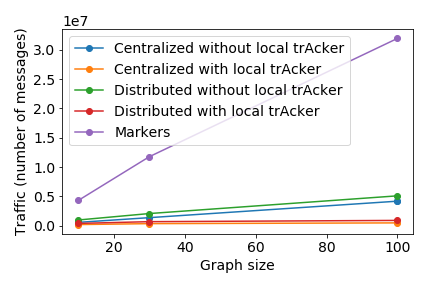
\includegraphics[width=0.99\textwidth]{pics/traffic_by_graph_size.png}
            \caption{Traffic by graph size}
    \end{subfigure}
    \hspace{5mm}
    \begin{subfigure}[b]{0.32\textwidth}
            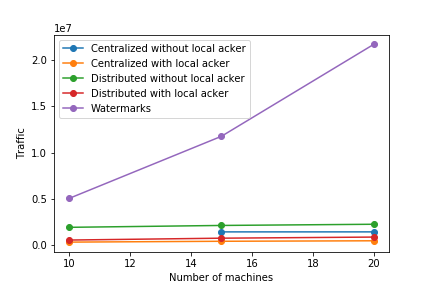
\includegraphics[width=0.99\textwidth]{pics/traffic_by_number_of_machines.png}
            \caption{Traffic by number of virtual machines}
    \end{subfigure}
    \hspace{5mm}
    \begin{subfigure}[b]{0.32\textwidth}
            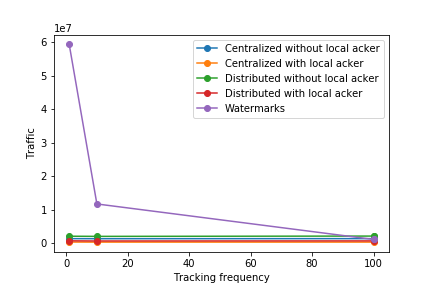
\includegraphics[width=0.99\textwidth]{pics/traffic_by_tracking_frequency.png}
            \caption{Traffic by tracking frequency}
	\end{subfigure}
    \caption{Service traffic of various trackings}
\end{figure*}

\subsubsection{Overhead on throughput} \label{overhead}

In those experiments we compare maximum throughput of system without tracking to systems with various trackings. \tracker's overhead on maximum throughput is not substantial and does not depend on tracking window frequency. Overhead of tracking with markers is huge when tracking every element.

\begin{figure}[htbp]
  \centering
  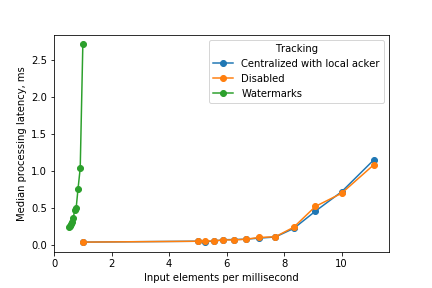
\includegraphics[width=0.50\textwidth]{pics/throughput_overhead.png}
  \caption{Throughput overhead}
\end{figure}

\subsection{Completeness monitoring} \label{completeness}

\subsubsection{Notification latency}

Notification latency was measured as a time between moments of Bench Stand receiving last elements in tracking windows and notifications for that window.

% https://gist.github.com/faucct/032aaf6240db361d30a184b1d7bf3c8e
\begin{figure*}[t!]
    \begin{subfigure}[b]{0.32\textwidth}
            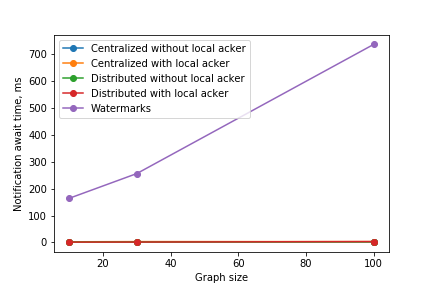
\includegraphics[width=0.99\textwidth]{pics/notification_await_time_by_graph_size.png}
            \caption{Notification latency by graph size}
    \end{subfigure}
    \hspace{5mm}
    \begin{subfigure}[b]{0.32\textwidth}
            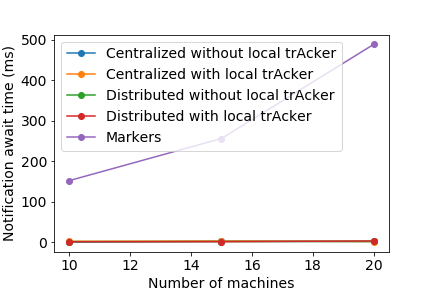
\includegraphics[width=0.99\textwidth]{pics/notification_await_time_by_number_of_machines.png}
            \caption{Notification latency by number of virtual machines}
    \end{subfigure}
    \hspace{5mm}
    \begin{subfigure}[b]{0.32\textwidth}
            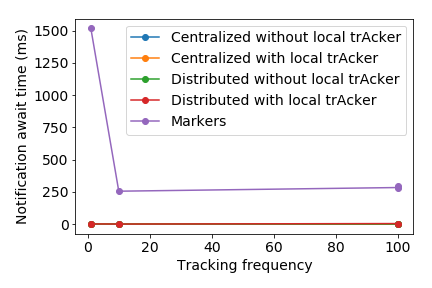
\includegraphics[width=0.99\textwidth]{pics/notification_await_time_by_tracking_frequency.png}
            \caption{Notification latency by tracking frequency}
	\end{subfigure}
    \caption{Notification latency of various trackings}
\end{figure*}

\subsubsection{Scalability}

In those experiments we are reproducing a case in which the centralized \tracker\ was not holding the load, while the distributed \tracker\ was working. We have failed to reproduce it while using 100 machines running our dataflow. Still, we have been able to simulate it by increasing the total number of Ack messages.

% https://gist.github.com/faucct/546f5617b958349a125449926373b780
\begin{figure}[htbp]
  \centering
  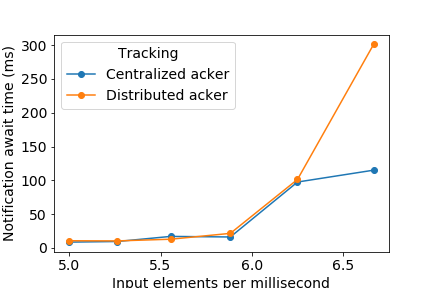
\includegraphics[width=0.50\textwidth]{pics/scalability_01x.png}
  \caption{1x acks}
\end{figure}
\begin{figure}[htbp]
  \centering
  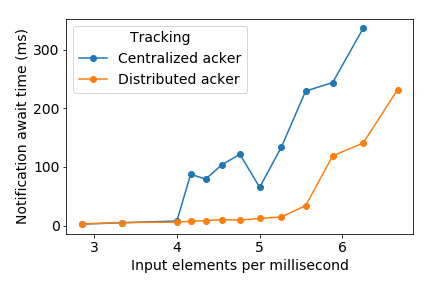
\includegraphics[width=0.50\textwidth]{pics/scalability_05x.png}
  \caption{5x acks}
\end{figure}
\begin{figure}[htbp]
  \centering
  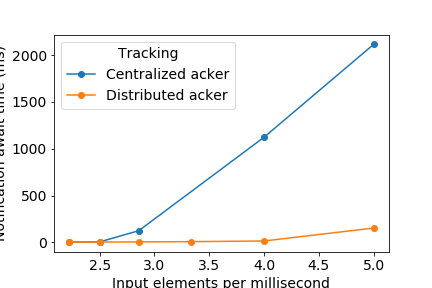
\includegraphics[width=0.50\textwidth]{pics/scalability_09x.png}
  \caption{9x acks}
\end{figure}
\begin{figure}[htbp]
  \centering
  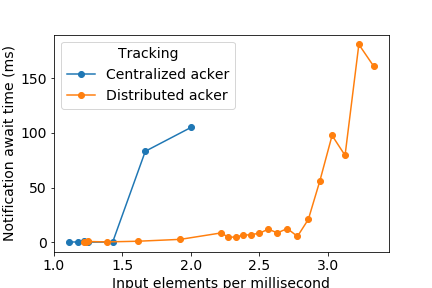
\includegraphics[width=0.50\textwidth]{pics/scalability_17x.png}
  \caption{17x acks}
\end{figure}

\subsection{State snapshotting} \label{snapshotting}

In those experiments we are comparing granular tracking using \tracker\ and markers. Processed elements are divided into snapshot windows. Pipeline vertices only process elements from a current snapshot window and buffer ones from a next snapshot window until they receive a notification that all elements from a current snapshot have been processed. When this happens vertices imitate snapshotting with a fixed duration sleep and continue to process elements from next snapshot window. We have measured a number of buffered elements and total time they have spent in buffer varying the snapshot duration.

% https://gist.github.com/faucct/6097d9d08197cb979b71721b16f8b6a3/
\begin{figure}[htbp]
  \centering
  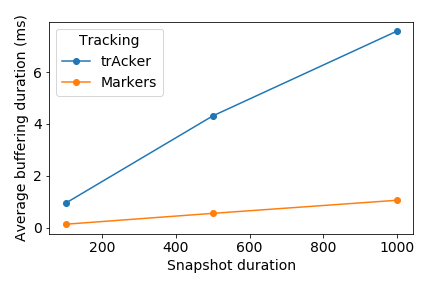
\includegraphics[width=0.50\textwidth]{pics/buffering_average_duration.png}
  \caption{Average buffering duration}
\end{figure}
\begin{figure}[htbp]
  \centering
  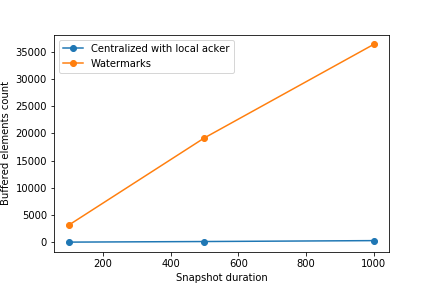
\includegraphics[width=0.50\textwidth]{pics/buffering_count.png}
  \caption{Buffered elements count}
\end{figure}
\begin{figure}[htbp]
  \centering
  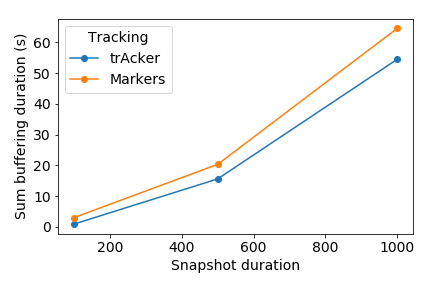
\includegraphics[width=0.50\textwidth]{pics/buffering_sum_duration.png}
  \caption{Total buffering duration}
\end{figure}
\begin{figure}[htbp]
  \centering
  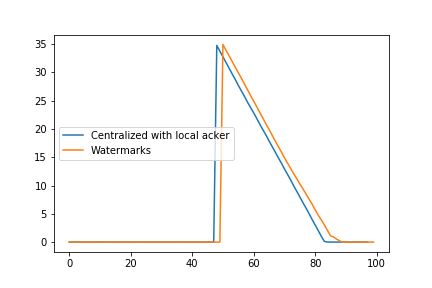
\includegraphics[width=0.50\textwidth]{pics/buffering_latencies_evolution_acker.png}
  \caption{Latencies with \tracker}
\end{figure}
\begin{figure}[htbp]
  \centering
  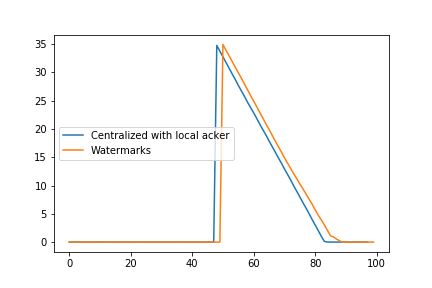
\includegraphics[width=0.50\textwidth]{pics/buffering_latencies_evolution_watermarks.png}
  \caption{Latencies with markers}
\end{figure}

\subsection{Count iterations?}

